\documentclass{ctexart}
\usepackage{listings} % 用于插入代码
\usepackage{graphicx} % 用于插入图片
\usepackage{amsmath}  % 用于数学公式
\usepackage{xcolor} % 用于代码高亮

\lstset{
  language=C, % 设置语言
  basicstyle=\small\ttfamily,
  numbers=left, % 在左侧显示行号
  numberstyle=\tiny\color{gray}, % 行号颜色
  stepnumber=1, % 行号增加步长
  numbersep=5pt, % 行号与代码的距离
  backgroundcolor=\color{white}, % 代码背景色
  showspaces=false, % 显示空格
  showstringspaces=false, % 字符串中显示空格
  showtabs=false, % 显示tab
  frame=single, % 显示边框
  rulecolor=\color{black}, % 边框颜色
  tabsize=2, % tab空格数
  captionpos=b, % 标题位置
  breaklines=true, % 自动折行
  breakatwhitespace=false, 
  escapeinside={\%*}{*)}, % 添加注释
  keywordstyle=\color{blue}, % 关键字颜色
  stringstyle=\color{red} % 字符串颜色
}

\title{Mandelbrot集合}
\author{Yoimiya}
\date{\today}

\begin{document}

\maketitle

\section{介绍}

Mandelbrot集合是一个在复平面上定义的点集。对于每一个复数$c$,如果从$z=0$开始的迭代$z_{n+1} = z_n^2 + c$不发散,那么$c$就属于Mandelbrot集合。Mandelbrot集合是分形的一个例子,它的边界具有无限的复杂性和自相似性。

Mandelbrot集合的形状是由一个简单的二次多项式生成的,但是它的边界却展示出了令人惊奇的复杂性和美丽。这个集合的每一部分都包含了无数的小型复制品,这些复制品和整个集合有着相同的形状。这种性质被称为自相似性,它是分形的一个重要特征。

Mandelbrot集合的另一个有趣的性质是它的无限性。无论你放大多少次,你总是能在集合的边界上发现新的细节。这种无限的复杂性和深度使得Mandelbrot集合成为了数学和艺术的一个重要主题。

Mandelbrot集合不仅仅是一个数学概念,它也是一个强大的视觉艺术工具。通过改变颜色和放大的程度,我们可以创建出各种各样的美丽图像。这些图像不仅仅展示了数学的美,也展示了自然界中无处不在的分形结构。

\section{历史}

Mandelbrot集合是由法国数学家本华·曼德布洛特在1980年首次定义的。他发现了这个集合的独特性质,并用计算机生成了它的图像。这个图像的美丽和复杂性引起了人们的广泛关注,使得分形成为了流行文化的一部分。

曼德布洛特在研究这个集合时,发现了一种全新的几何形态,这种形态既不是欧几里得几何,也不是非欧几里得几何,而是一种全新的、复杂的、自相似的几何形态。他将这种几何形态称为"分形",并用它来描述自然界中的许多现象,如云朵、山脉、树木等。

曼德布洛特的发现引起了科学界的广泛关注。他的工作不仅改变了我们对几何的理解,也为许多领域,如物理学、生物学、计算机科学等,提供了新的研究工具。今天,分形已经成为了现代科学的一个重要部分,而Mandelbrot集合则是分形的最著名的例子。

尽管Mandelbrot集合的定义非常简单,但是它的边界却展示出了无穷的复杂性。这种从简单规则中产生的复杂性是分形的一个重要特征,也是Mandelbrot集合的一个重要的历史贡献。

\section{性质}

Mandelbrot集合的一个重要性质是它的自相似性。也就是说,如果你放大Mandelbrot集合的一部分,你会看到和整个集合类似的形状。这种性质使得Mandelbrot集合具有无限的复杂性,即使在任意小的尺度上,都可以看到新的细节。

Mandelbrot集合的另一个重要性质是它的连通性。在复平面上,所有属于Mandelbrot集合的点都是连通的,也就是说,你可以从任何一个点走到任何其他的点,而不需要离开集合。

此外,Mandelbrot集合的边界是一个分形。这意味着它的边界具有无限的复杂性和自相似性。无论你放大多少次,你总是能在边界上发现新的细节和结构。

Mandelbrot集合的这些性质使得它在数学和物理学中有许多应用。例如,它被用来模拟自然界中的许多现象,如云朵的形状、山脉的轮廓、树木的分支等。同时,它也是一个强大的视觉艺术工具,可以用来创建美丽的图像和动画。

\section{代码}

以下是计算Mandelbrot集合的一个简单的代码模板:

\begin{lstlisting}[language=C]
#include <stdio.h>

// 计算Mandelbrot集合的函数
// 输入:real和imag分别表示复数的实部和虚部
// 输出:返回一个整数,表示该点是否属于Mandelbrot集合,以及它的迭代次数
int mandelbrot(double real, double imag) {
    int max_iter = 1000; // 最大迭代次数,增加这个值可以增加图像的细节
    double r = 0.0; // 初始化复数的实部
    double i = 0.0; // 初始化复数的虚部
    int n = 0; // 初始化迭代次数
    // 迭代计算,直到超过最大迭代次数或者复数的模大于2
    for(; n < max_iter && r*r + i*i <= 4.0; n++) {
        double temp = r*r - i*i + real; // 计算下一个实部
        i = 2*r*i + imag; // 计算下一个虚部
        r = temp;
    }

    // 平滑颜色算法
    if (n == max_iter) {
        return 0; // 如果点在Mandelbrot集合中,返回0表示黑色
    } else {
        // 如果点不在Mandelbrot集合中,使用平滑颜色算法计算颜色
        // 这个算法可以使颜色的变化更加平滑,而不是突变
        double zn = sqrt(r * r + i * i);
        int nu = log2(1.75 + log2(log2(zn))) / log2(2);
        n = n + 1 - nu;
        return n;
    }
}

// 颜色映射函数
// 输入:一个整数,表示点是否属于Mandelbrot集合以及它的迭代次数
// 输出:一个RGBTRIPLE结构,表示该点的颜色
void color_map(int value, RGBTRIPLE* color) {
    if (value == 0) {
        // 如果点在Mandelbrot集合中,颜色为黑色
        color->rgbRed = 0;
        color->rgbGreen = 0;
        color->rgbBlue = 0;
    } else {
        // 如果点不在Mandelbrot集合中,根据迭代次数计算颜色
        // 这个算法可以生成各种各样的颜色,你可以根据需要修改它
        color->rgbRed = value % 8 * 32;
        color->rgbGreen = value % 16 * 16;
        color->rgbBlue = value % 32 * 8;
    }
}
\end{lstlisting}

\section{结果}

以下是使用上述代码生成的Mandelbrot集合的图像:

\begin{figure}[h]
    \centering
    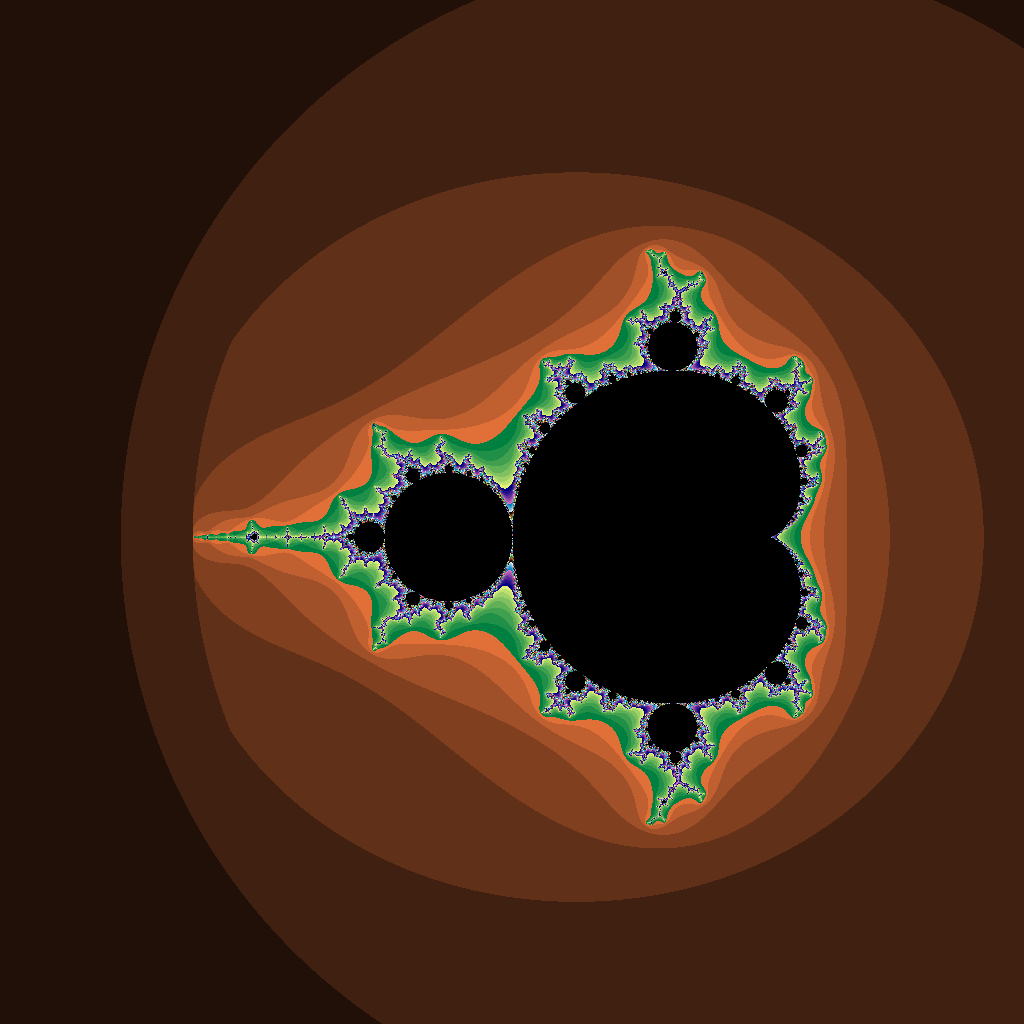
\includegraphics[width=1.0\textwidth]{mandelbrot.png}
    \caption{Mandelbrot集合}
\end{figure}

\end{document}